% !TeX program = xelatex
\documentclass[aspectratio=169]{beamer}
\usepackage{etex} % fixes new-dimension error
%-------------- template --------------------------------------------------
\usetheme{metropolis}
\metroset{block=fill}

% Configuring the foot line
\setbeamertemplate{footline}
{
  \leavevmode%
  \hbox{%
  \begin{beamercolorbox}[wd=.4\paperwidth,ht=2.25ex,dp=1ex,center]{author in head/foot}%
    \usebeamerfont{author in head/foot}\insertshortauthor
  \end{beamercolorbox}%
  \begin{beamercolorbox}[wd=.5\paperwidth,ht=2.25ex,dp=1ex,center]{title in head/foot}%
    \usebeamerfont{title in head/foot}\insertsection
  \end{beamercolorbox}%
  \begin{beamercolorbox}[wd=.1\paperwidth,ht=2.25ex,dp=1ex,right]{date in head/foot}%
    \insertframenumber{} / \inserttotalframenumber\hspace*{2ex} 
  \end{beamercolorbox}}%
  \vskip0pt%
}
\makeatother
\setbeamertemplate{navigation symbols}{}
%----------------------------------------------------------------------------
\usepackage{graphicx,amsmath}
\usepackage{stmaryrd} % cf. interleave
\usepackage{booktabs}
\usepackage{amscd}
\usepackage{multicol}
\usepackage[absolute,overlay]{textpos}
\usepackage{alltt}
\usepackage{proof}
\usepackage{tikz}
\usepackage{cancel}
\usepackage{mathrsfs}  
\usepackage{relsize}
\usepackage[all]{xy}
\usetikzlibrary{tikzmark,arrows.meta,calc}

\AtBeginSection[]
{
    \begin{frame}
        \frametitle{Table of Contents}
        \tableofcontents[currentsection]
    \end{frame}
}

\author[Renato Neves]{Renato Neves}

% logos of institutions
\titlegraphic{
  \begin{textblock*}{5cm}(11cm,7.45cm)
     
\includegraphics[scale=0.044]{images/uminho.png}\hspace*{.85cm}~%
  \end{textblock*}
  \begin{textblock*}{5cm}(13cm,7.45cm)
    
\includegraphics[scale=0.4]{images/haslab.pdf}
  \end{textblock*}
}

\input{macros}
% No date
\date{}

\newenvironment{mexamples}
  {\begin{exampleblock}{Examples}}
  {\end{exampleblock}}

\begin{document}

\title{Hoare Logic}
\frame[plain]{\titlepage}

\begin{frame}[plain]

        \begin{textblock*}{5cm}(11cm,1.5cm)
            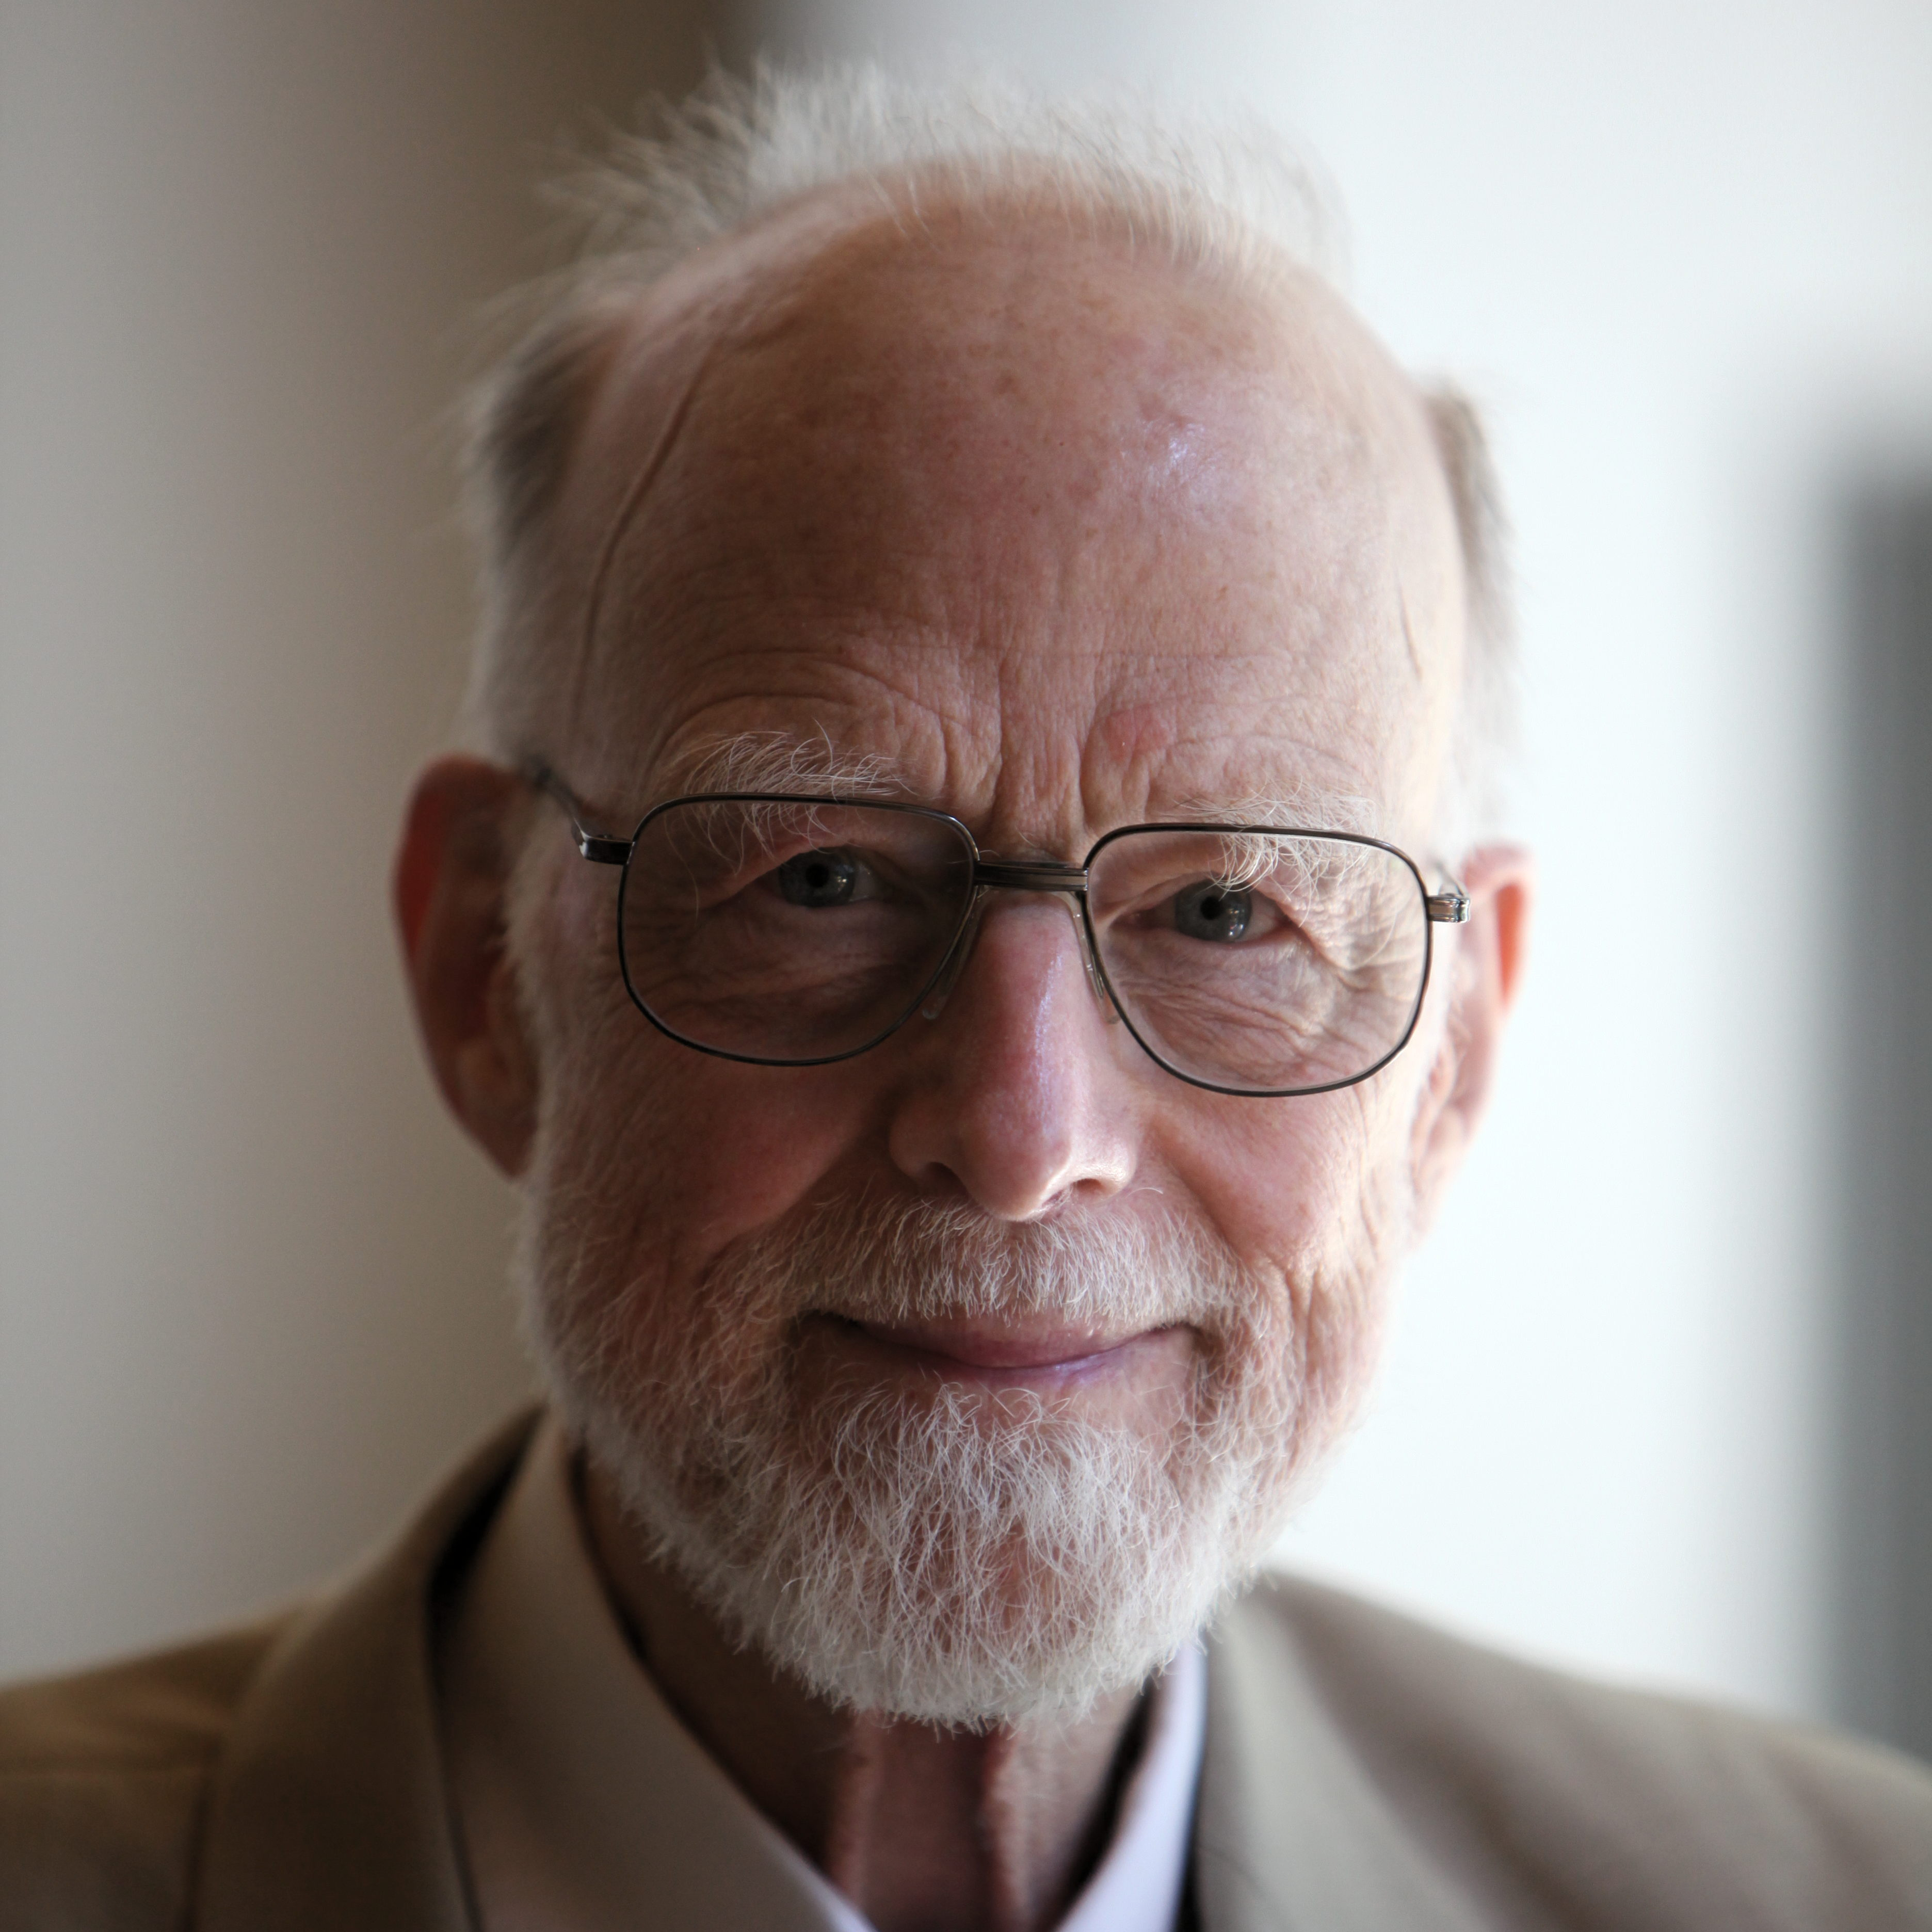
\includegraphics[scale=0.03]{images/hoare.jpg}\hspace*{.85cm}~%
        \end{textblock*}

        \vspace{5cm}
        \large{
                \dots \, or \dots \, the \salert{science} of knowing whether
                \salert{bugs} will make my plane \salert{crash}
        }
\end{frame}

\begin{frame}{The protagonist}
        \[
            \Large
            \tikzmarknode{hoare}{  \{ \Phi \} \, P \, \{ \Psi \}  }
        \]

        \begin{tikzpicture}[remember picture,overlay]
                \draw[<-,thick,red] (hoare.south)+(0.0,-0.2)  -- ++(0.0,-0.5)
                        -- ++(0.0,-0.25)
                        node[below]{\footnotesize Hoare triple};
        \end{tikzpicture}


         \pause
         \vfill
         \begin{center}
                notation for ``input has \salert{property} $\Phi$
                $\Longrightarrow$ output has \salert{property} $\Psi$"
         \end{center}
\end{frame}

\begin{frame}{A fistful of Hoare triples}
       
        \begin{mexamples}
        \begin{itemize} 
                \item $\{ \text{ ``list is valid'' } \} 
                      \, \mathbf{QuickSort} \, 
                      \{ \text{ ``list is ordered'' } \}$
                %
                \item $\{ \text{ ``list is valid and x is valid'' } \}
                      \, \mathbf{Insert} \, 
                      \{ \text{ ``x is in the list'' } \}$
                \item $\{ \text{ ``normal initial parameters'' } \} 
                      \, \mathbf{Plane} \, 
                      \{ \text{ ``altitude is (mostly) safe'' } \}$
                \item $\{ \text{ ``list is valid and x is in the list'' } \} 
                        \, \mathbf{QuantumFind} \, 
                      \{ \text{ ``(frequently) true'' } \}$
        \end{itemize}
        \end{mexamples}
        %
        \pause
        \vfill
        \begin{center}
                \fbox{But how to describe such properties \salert{rigorously} ?}
        \end{center}
\end{frame}

\begin{frame}{The failure of natural language}

        \begin{itemize}
                \item ``Ninguém para o Braga''
                \item ``O Salazar sentou-se na cadeira e partiu a perna''
                \item ``Brexit does mean Brexit''
                \item ``Don't worry -- this plane is mostly safe !''
        \end{itemize}
\end{frame}

\section{First-order logic (FOL)}

\begin{frame}{Our old friend, first-order logic, to the rescue}

        Rigorous

        Deceptively simple

        Powerful enough to handle a large portion of \salert{mathematics}
\end{frame}


\begin{frame}{The basic ingredients}

        Typed variables (\ie\ placeholders) $x : \typeA$

        Typed operations (\eg\ addition) $f : \typeA_1, \dots, \typeA_n \to \typeA$

        Predicates (\eg\ equality) $p : \typeA_1, \dots, \typeA_n$

        Boolean connectives $\wedge, \Rightarrow, \neg$

        \salert{Quantifiers} $\forall x : \typeA. \, \dots, \exists x : \typeA. \, \dots$

        \pause
        \vspace{0.5cm}
        \dots\ plus a set of rules that underlie human reasoning and advanced
        PLs -- and which hopefully you will see in later courses ;-)
\end{frame}

\begin{frame}{From natural language to FOL}
        Let's translate the following sentences to FOL (\ie\ first-order logic)
        %
        \begin{enumerate}
                \item $m$ is an upper bound of $x$ and $y$
                \item $m$ is the maximum of $x$ and $y$
                \item all natural numbers are either odd or even
                \item there exists no real number that is equal
                        to the square root of $-1$
                \item $i$ is the largest number for which predicate $\phi : \Nats$
                        holds
                \item every nat. nº greater than $2$ is the sum
                        of two prime nºs  (\salert{Golbach's conjecture})
        \end{enumerate}
\end{frame}

\begin{frame}{A word of warning -- specifications vs implementations}

        FOL is a logic for reasoning about \, \dots \, properties
        (\salert{specifications})

        A programming language is a language for \, \dots \, programming
        (\salert{implementations})

        Don't try to program in FOL neither to specify in \texttt{C}

        \pause
        \vfill
        Let's go the exercise sheet !!
\end{frame}
\end{document}
